
\begin{figure}
    \centering
    \includegraphics[width=0.92\textwidth]{images/mass_effect3_smoke.jpg}
    \caption{Animação de fumaça no jogo \textit{Mass Effect 3}.}
    \subcaption*{Fonte: \url{https://www.fxguide.com/fxfeatured/cinematics-case-study-mass-effect-3/}}
    \label{fig:masseffect3}
\end{figure}

As indústrias do entretenimento, jogos (\figref{fig:masseffect3}) e engenharia têm grande interesse em simulações de fluidos para integrar em seus respectivos produtos. Em geral, simulações baseadas em física tendem a apresentar resultados visualmente realísticos e convincentes, podendo levar uma pessoa leiga na área a confundir uma gravação real com uma simulação \cite{Huang2015}. É necessário que o observador da simulação seja convencido da sua veracidade, pois isso aumenta a imersão na experiência de um filme ou jogo. Para alcançar esse nível de qualidade desejado, é preciso trabalhar com técnicas computacionalmente custosas, para perder o mínimo de detalhes possível na simulação. Portanto, é importante utilizar métodos com alta precisão e otimização do tempo de execução, para poder aplicar a técnica em tempo real, no caso de jogos, e poupar tempo na produção de efeitos especiais em filmes.

O comportamento de fluidos no mundo real é descrito de maneira contínua. Quando se discretiza este fenômeno para simular computacionalmente, é necessário realizar um passo de discretização do domínio. Por conta disto, simulações de fluidos podem ser abordadas de duas maneiras mais comumente usadas: visão lagrangiana e visão euleriana, além da forma híbrida.

Na visão lagrangiana (ver \figref{fig:lagrangiana}), o fluido é discretizado em forma de um sistema de partículas, com cada uma delas representando uma parte da massa fluídica (volume). Cada partícula tem uma posição no domínio e carrega consigo algumas propriedades daquela parte do fluido que a mesma está discretizando, como velocidade, posição, pressão e força externa. A simulação é realizada pela determinação, em cada passo de tempo, da posição e velocidade de cada partícula do sistema. Já na abordagem euleriana (ver \figref{fig:euleriana}), a discretização do espaço é feita em uma grade ou malha. Esta grade é dividida em células, e estas armazenam as propriedades do fluido que estão passando por aquela região do espaço, sendo responsáveis por gerir como o fluido irá escoar.

\begin{figure}
    \centering
    \caption{Tipos de simulações de escoamento de fluidos}
    \begin{subfigure}[b]{0.45\textwidth}
        \centering
        \includegraphics[width=\textwidth]{images/lagrangeana.pdf}
        \caption{Simulação pela visão lagrangiana.}
        \label{fig:lagrangiana}
    \end{subfigure}
    \hfill
    \begin{subfigure}[b]{0.45\textwidth}
        \centering
        \includegraphics[width=\textwidth]{images/euleriana.pdf}
        \caption{Simulação pela visão euleriana.}
        \label{fig:euleriana}
    \end{subfigure}
    \subcaption*{Fonte: Elaborada pelo autor.}
    \label{fig:simulacoes}
\end{figure}

Existem diversas características que diferem na representação da malha. Por exemplo, existem malhas regulares e irregulares. Em malhas regulares, os centros de cada célula são equidistantes e colineares, enquanto nas malhas irregulares não existe esta restrição. Outro fator que pode distinguir é a topologia de cada célula da malha: existem malhas com topologia tetraédrica, hexaédrica ou mistas. Malhas tetraedrais se moldam melhor em fronteiras irregulares, como objetos complexos, porém, este benefício é contrabalançado pelo grande custo computacional. Malhas hexaédricas têm a desvantagem de perder muitos detalhes por conta da estrutura simples. Grades híbridas têm a vantagem de poder usar células tetraédricas em fronteiras com objetos complexos, e células hexaédricas em espaços abertos, melhorando o custo computacional \cite{Huang2015}. Além disso, os valores do campo escalar ou campo vetorial podem ser armazenados no centro de cada célula ou no centro de cada face. Caso ambos estejam no centro, esta malha é chamada de co-localizada (do inglês, \textit{collocated}), e no caso do campo escalar estar no centro da célula e a velocidade na face, esta malha é chamada de deslocada (do inglês, \textit{staggered}), conforme ilustrado na \figref{fig:celulas}. O foco do nosso trabalho será a simulação de fluidos por meio da abordagem euleriana com uso de malhas tetraedrais deslocadas.

\begin{figure}
    \centering
    \caption{Tipos de células presentes na abordagem euleriana em duas dimensões.}
    \begin{subfigure}[b]{0.23\textwidth}
        \centering
        \includegraphics[width=\textwidth]{images/quad_collocated.pdf}
        \caption{Célula quadricular co-localizada.}
        \label{fig:quadcollo}
    \end{subfigure}
    \hspace{0.1\textwidth}
    \begin{subfigure}[b]{0.23\textwidth}
        \centering
        \includegraphics[width=\textwidth]{images/quad_staggered.pdf}
        \caption{Célula quadricular deslocada.}
        \label{fig:quadstagg}
    \end{subfigure}
    \newline
    \begin{subfigure}[b]{0.23\textwidth}
        \centering
        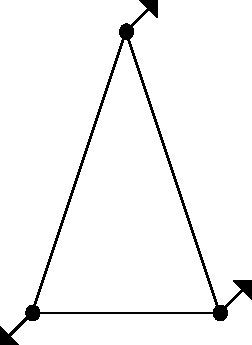
\includegraphics[width=\textwidth]{images/tri_collocated.pdf}
        \caption{Célula triangular co-localizada.}
        \label{fig:tricollo}
    \end{subfigure}
    \hspace{0.1\textwidth}
    \begin{subfigure}[b]{0.23\textwidth}
        \centering
        \includegraphics[width=\textwidth]{images/tri_staggered.pdf}
        \caption{Célula triangular deslocada.}
        \label{fig:tristagg}
    \end{subfigure}
    \subcaption*{Fonte: Elaborada pelo autor.}
    \label{fig:celulas}
\end{figure}

Em geral, simulações de fluidos baseadas em física têm como base as Equações de Navier-Stokes (ENS) para fluidos incompressíveis \cite{incompressible}. Estas são um conjunto de equações diferenciais parciais que descrevem o escoamento dos fluidos. Para resolver as ENS, é necessária a aplicação de operadores diferenciais de cálculo vetorial, tais como: gradiente, divergente e laplaciano. Estes operadores são aplicados em funções contínuas; no entanto, não é possível representar funções contínuas em computadores, logo, estas devem ser discretizadas. Na abordagem euleriana, o método de Diferenças Finitas (do inglês, \textit{Finite Differences} - FD) visa solucionar este problema para grades uniformes. A aplicação de FD em uma célula da grade necessita acessar informações dos vizinhos; estes vizinhos são chamados de estêncil, no caso 2D são 4 e no 3D são 6, conforme mostrado na \figref{fig:stencils}. Como esta vizinhança é fixa em grades uniformes, podemos aplicar este método de forma eficiente.

\begin{figure}
    \centering
    \caption{Tipos de estênceis em grades uniformes.}
    \begin{subfigure}[b]{0.23\textwidth}
        \centering
        \includegraphics[width=\textwidth]{images/stencil-2d.pdf}
        \caption{Estêncil 2D.}
        \label{fig:2dsten}
    \end{subfigure}
    \hspace{0.1\textwidth}
    \begin{subfigure}[b]{0.23\textwidth}
        \centering
        \includegraphics[width=\textwidth]{images/stencil-3d.pdf}
        \caption{Estêncil 3D.}
        \label{fig:3dsten}
    \end{subfigure}
    \subcaption*{Fonte: Elaborada pelo autor.}
    \label{fig:stencils}
\end{figure}

Quando trabalhamos com malhas tetraedrais, temos que aceitar uma malha não-estruturada. Esta propriedade impossibilita o uso de FD, pois a vizinhança de uma célula não é fixa, sendo necessário o uso de outros métodos para a resolução destes operadores diferenciais em malhas não-estruturadas, tais como os métodos de Elementos Finitos e Volumes Finitos. Em animação computacional, o método de Volumes Finitos (do inglês, \textit{Finite Volumes} - FV) é o mais utilizado para animação de fumaça em malhas não-estruturadas \cite{Klingner2006}.

Outra propriedade importante de malhas que deve ser considerada é a conformidade, que consiste na topologia da mesma. Uma malha conforme (ver \figref{fig:conforme}) contém todas as arestas da face completa, ou seja, não existe um vértice que resida no interior de uma aresta. Na literatura, encontramos diversos problemas geométricos \cite{Mahmood2019, nonconf1} em malhas não-conformes (ver \figref{fig:africa}). No entanto, há uma lacuna na resolução das ENS nesse tipo de malha. Para resolver numericamente as ENS, é interessante utilizar um método que seja independente da malha, isto é, métodos de interpolação sem malha.

\begin{figure}
    \centering
    \caption{Exemplo de malha conforme.}
    \includegraphics[width=0.7\textwidth]{images/africa-conforme.jpg}
    \subcaption*{Fonte: \cite{Nascimento:2014}}
    \label{fig:conforme}
    \vspace{-1.2cm}
\end{figure}

\begin{figure}
    \centering
    \caption{Exemplo de malha não-conforme, com círculo vermelho para evidenciar uma aresta que mostra a propriedade da malha.}
    \includegraphics[width=0.7\textwidth]{images/africa-nao-conforme.png}
    \subcaption*{Fonte: Adaptado de \cite{Nascimento:2014}}
    \label{fig:africa}
\end{figure}

O método baseado em Funções de Base Radial (do inglês, \textit{Radial Basis Function} - RBF) \cite{rbf} faz uma interpolação independente de malha, e sua aproximação de FD conhecida como \textit{Radial Basis Function Finite Differences} (RBF-FD) \cite{WRIGHT200699}, resolve os operadores diferenciais necessários. Logo, com a aplicação do RBF-FD em malhas não-conformes, pretendemos resolver as ENS e representar visualmente a simulação da fumaça.

\section{Objetivos}

O objetivo principal deste trabalho é desenvolver uma técnica eficiente de animação de fumaça em malhas não-estruturadas utilizando o método RBF-FD, abordando as limitações atuais na aplicação de condições de contorno em malhas tetraedrais.


\section{Roteiro}

O resto do texto se divide da seguinte maneira. No capítulo \ref{chapter:revisao}, abordaremos como evoluiu a simulação de fluidos computacional ao longo do tempo, avaliando os métodos canônicos até os métodos mais atuais. No capítulo \ref{chapter:fundteorica} demonstraremos a fundamentação teórica que basea nossa solução e enunciar os problemas a serem resolvidos. No capítulo \ref{chapter:metodologia}, explicaremos os principais métodos utilizados na nossa pesquisa, como o RBF-FD, e como aplicar as condições de contorno de Neumann neste caso. Por fim, No capítulo \ref{chapter:Resultados}, daremos um contexto geral do nosso projeto, explicitando as expectativas, hipóteses e o cronograma para o desenvolvimento do projeto.
